\documentclass{article}
\usepackage[margin=0in]{geometry}
\usepackage{orne1}
\usepackage{plotjour1}
\begin{document}
  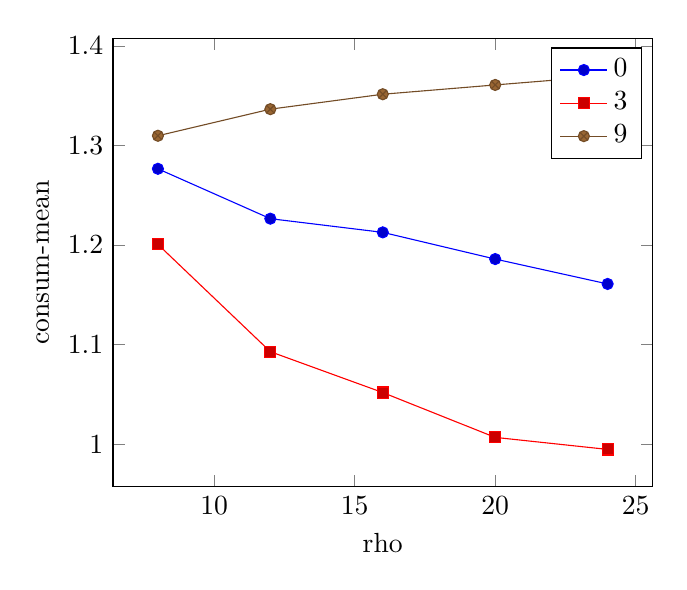
\begin{tikzpicture}
    \begin{axis} [
      xlabel = { rho}, 
      ylabel = { consum-mean}
      ]
      \addplot coordinates {
        (8, 1.27648879367831)
        (12, 1.22641079582322)
        (16, 1.21267156909354)
        (20, 1.18585272162843)
        (24, 1.16086806675415)};
      \addplot coordinates {
        (8, 1.20058264073122)
        (12, 1.09284072844579)
        (16, 1.05181239451852)
        (20, 1.00678600574349)
        (24, 0.994714262261039)};
      \addplot coordinates {
        (8, 1.30966322916668)
        (12, 1.33637318536933)
        (16, 1.35137219010417)
        (20, 1.36070642680922)
        (24, 1.36987739062501)};
      \legend{{0}, {3}, {9}}%
    \end{axis}
  \end{tikzpicture}
  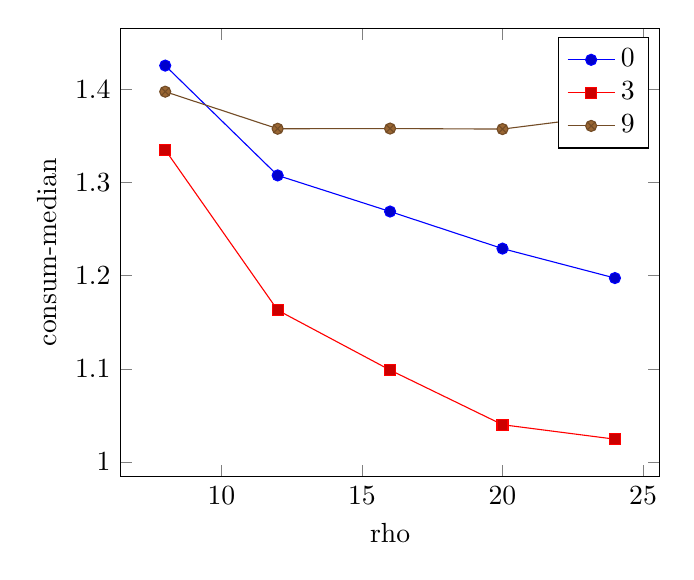
\begin{tikzpicture}
    \begin{axis} [
      xlabel = { rho}, 
      ylabel = { consum-median}
      ]
      \addplot coordinates {
        (8, 1.42567896804059)
        (12, 1.30774666499467)
        (16, 1.26896156363169)
        (20, 1.22916003071137)
        (24, 1.19753021391977)};
      \addplot coordinates {
        (8, 1.33520471208897)
        (12, 1.16303433353963)
        (16, 1.09872415146094)
        (20, 1.04006662943248)
        (24, 1.0245203704575)};
      \addplot coordinates {
        (8, 1.39765421875001)
        (12, 1.35785171875)
        (16, 1.35806078125)
        (20, 1.35750046875)
        (24, 1.37273890625001)};
      \legend{{0}, {3}, {9}}%
    \end{axis}
  \end{tikzpicture}

  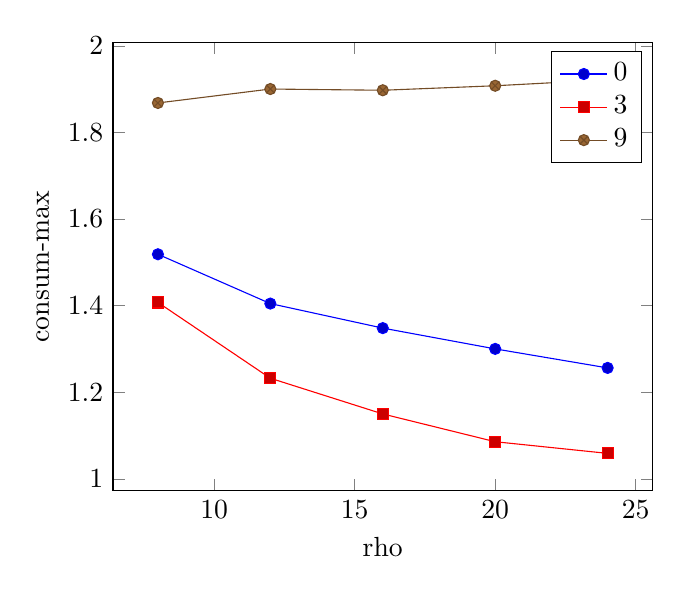
\begin{tikzpicture}
    \begin{axis} [
      xlabel = { rho}, 
      ylabel = { consum-max}
      ]
      \addplot coordinates {
        (8, 1.51863069522997)
        (12, 1.40471956575389)
        (16, 1.34810972950113)
        (20, 1.30010010901446)
        (24, 1.25620575188984)};
      \addplot coordinates {
        (8, 1.40742181660598)
        (12, 1.23233764339578)
        (16, 1.14987865196844)
        (20, 1.08574299302449)
        (24, 1.05882925201912)};
      \addplot coordinates {
        (8, 1.86802828125007)
        (12, 1.90018851562508)
        (16, 1.89735625000009)
        (20, 1.90774804687509)
        (24, 1.92153906250009)};
      \legend{{0}, {3}, {9}}%
    \end{axis}
  \end{tikzpicture}
  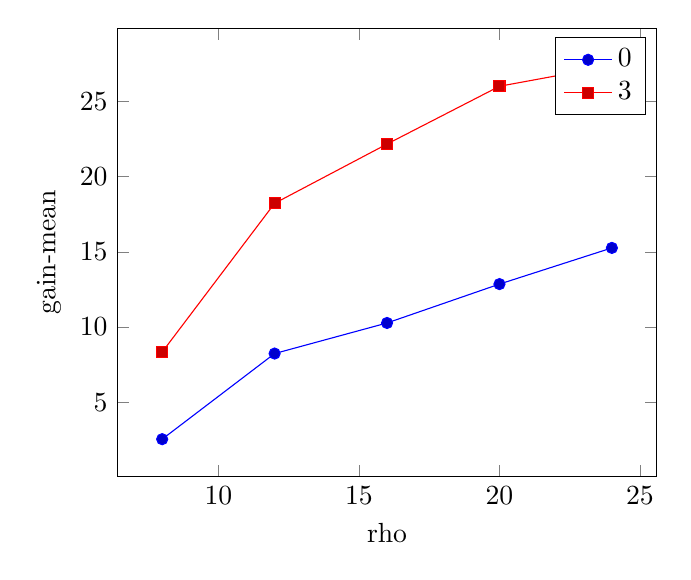
\begin{tikzpicture}
    \begin{axis} [
      xlabel = { rho}, 
      ylabel = { gain-mean}
      ]
      \addplot coordinates {
        (8, 2.53305084464157)
        (12, 8.22841933301131)
        (16, 10.2636876817732)
        (20, 12.8502152805151)
        (24, 15.2575205125107)};
      \addplot coordinates {
        (8, 8.32890364531846)
        (12, 18.2233869692794)
        (16, 22.1670830419087)
        (20, 26.0100499338167)
        (24, 27.3866209437036)};
      \legend{{0}, {3}}%
    \end{axis}
  \end{tikzpicture}

  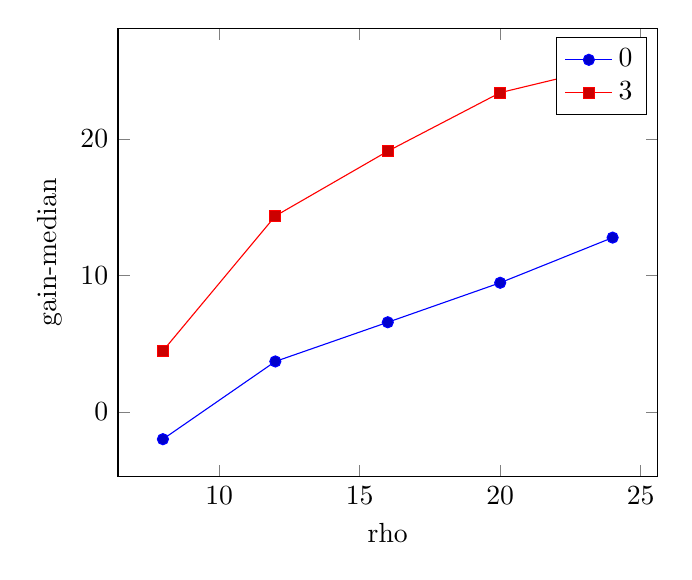
\begin{tikzpicture}
    \begin{axis} [
      xlabel = { rho}, 
      ylabel = { gain-median}
      ]
      \addplot coordinates {
        (8, -2.0051275139888)
        (12, 3.69002395942425)
        (16, 6.5607680339831)
        (20, 9.45417264988569)
        (24, 12.76343895642)};
      \addplot coordinates {
        (8, 4.46816571819157)
        (12, 14.3474712680496)
        (16, 19.0960988911235)
        (20, 23.3837001625365)
        (24, 25.3666982269599)};
      \legend{{0}, {3}}%
    \end{axis}
  \end{tikzpicture}
  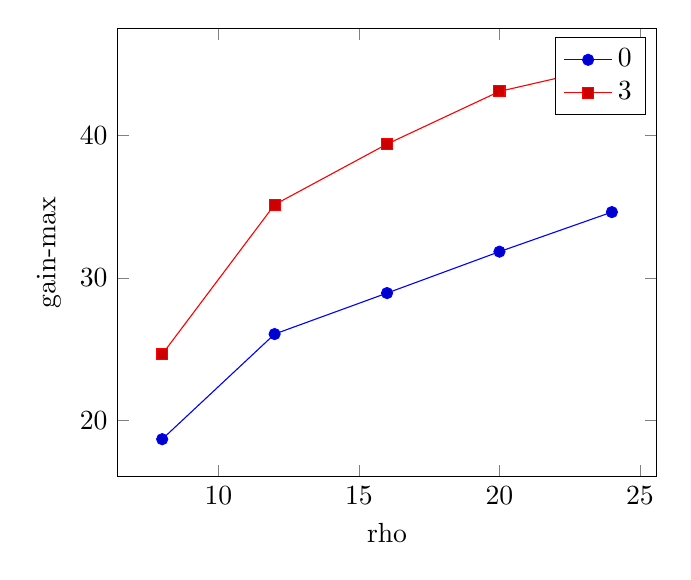
\begin{tikzpicture}
    \begin{axis} [
      xlabel = { rho}, 
      ylabel = { gain-max}
      ]
      \addplot coordinates {
        (8, 18.7040843828281)
        (12, 26.0747260493889)
        (16, 28.9479912113993)
        (20, 31.851582228375)
        (24, 34.6250213484907)};
      \addplot coordinates {
        (8, 24.6573603444515)
        (12, 35.1465587091821)
        (16, 39.3957433155534)
        (20, 43.0877156549606)
        (24, 44.8968135656068)};
      \legend{{0}, {3}}%
    \end{axis}
  \end{tikzpicture}

\end{document}